\documentclass[12pt]{article}
\usepackage{geometry}                % See geometry.pdf to learn the layout options. There are lots.
\geometry{letterpaper}                   % ... or a4paper or a5paper or ... 
\usepackage{graphicx}
\usepackage{amssymb}
\usepackage{amsthm}
\usepackage{epstopdf}
\usepackage[utf8]{inputenc}
\usepackage[usenames,dvipsnames]{color}
\usepackage[table]{xcolor}
\usepackage{hyperref}
\DeclareGraphicsRule{.tif}{png}{.png}{`convert #1 `dirname #1`/`basename #1 .tif`.png}

\theoremstyle{definition}
\newtheorem{example}{Example}

\newcommand{\projectname}{Smart Shopping List}
\newcommand{\productname}{Smart Shopping List}
\newcommand{\projectleader}{A. Walliser}
\newcommand{\documentstatus}{In process}
%\newcommand{\documentstatus}{Submitted}
%\newcommand{\documentstatus}{Released}
\newcommand{\version}{V. 1.0}

\begin{document}
\begin{titlepage}
\begin{flushright}

\includegraphics[scale=.5]{htlleondinglogo.png}\\
\end{flushright}

\vspace{10em}

\begin{center}
{\Huge System Specification} \\[3em]
{\LARGE \productname} \\[3em]
\end{center}

\begin{flushleft}
\begin{tabular}{|l|l|}
\hline
Project Name & \projectname \\ \hline
Project Leader & \projectleader \\ \hline
Document state & \documentstatus \\ \hline
Version & \version \\ \hline
\end{tabular}
\end{flushleft}

\end{titlepage}
\section*{Revisions}
\begin{tabular}{|l|l|l|}
\hline
\cellcolor[gray]{0.5}\textcolor{white}{Date} & \cellcolor[gray]{0.5}\textcolor{white}{Author} & \cellcolor[gray]{0.5}\textcolor{white}{Change} \\ \hline
November 29, 2018&C. Wagner/A. Walliser&First version \\ \hline
\end{tabular}
\pagebreak

\tableofcontents
\pagebreak

\section{Initial Situation and Goal}

\subsection{Initial Situation}

Members of a typical household must go shopping for groceries at least once a week. A lot of households use grocery lists to organise that process. Problems that could occur are that the grocery list gets lost or if the list is in use nobody else can add shopping items to the list. It also could happen that multiple lists get written because of miscommunication between the members of a household.

Furthermore things get more complex when the combination of recipe books and grocery lists is considered. The items found in different recipe books have to be manually transferred to the shopping list. 

These processes could be simplified by using a grocery list app.

\subsubsection{Application Domain}
Most people write a shopping list before they go shopping. When one member of a household goes shopping they only buy the products they wrote down. To not forget a product they have to communicate with every member of the household and ask them which items they want. Furthermore the items are written down in the order the writer is thinking of them, but in the store they want the items to be sorted according to the departments they belong to. 
\subsubsection{Glossary}

\subsubsection{Model of the Application Domain}

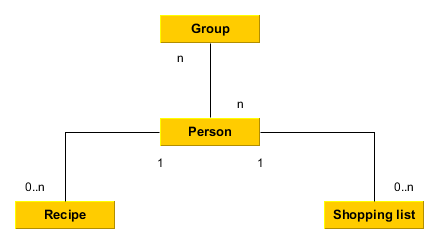
\includegraphics[scale=.5]{AppDomain.png}

\subsection{Goal Definition}

The main goal of our system is to speed up and simplify the process of going shopping and storing recipes. We especially want to help people living and shopping together so they need to spend less time talking about groceries. The system also helps managing and sharing ones recipes and lists because it is way more unlikely to lose or misplace ones recipes and shopping lists.
Our target group is every person that goes shopping but we especially want to cater to households with multiple members.

\pagebreak

\section{Functional Requirements}

\subsection{Use-Case Diagrams}

\subsection{Use Case Store Recipe}

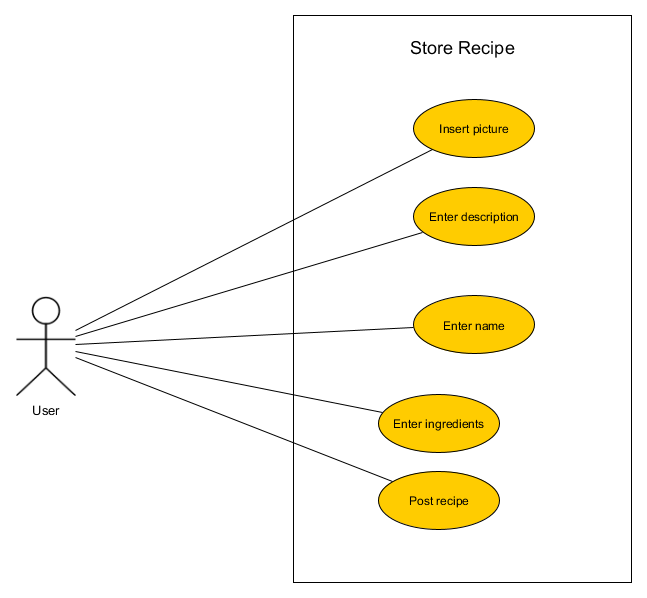
\includegraphics[scale=.5]{UseCaseStoreRecipe.png}\\

\subsection{Store Recipe Use Case Details}

Store recipe can be used in single-user and group-mode. If a recipe is created and stored while in group-mode the recipe will automatically be added to ones personal recipe book. A picture can be added to recipe to display the looks of ones dish. When a recipe is stored a name has to be assigned. Ingredients are split into needed ingredients and optional ingredients. The user can give the recipe a description in order to write down how to cook their recipe. After a recipe is stored it can be posted to make it accessible for other users.

\subsubsection{Characteristic Information}

\begin{tabular}{|l|l|}
\hline
Goal & Creates a recipe that is added to the users recipelist  \\ \hline
Involved User & The user who wants to create a recipe \\ \hline
\end{tabular}

\subsubsection{GUI to call the use case}

\begin{tabular}{|l|l|}
\hline
Input field & Valid inputs \\ \hline
 &  \\ \hline
\end{tabular}

\subsubsection{Scenario for the standard use}

\begin{tabular}{|l|l|l|}
\hline
Step & User & Activity \\ \hline
 & & \\ \hline
\end{tabular}

\subsubsection{GUIs for the standard use}

\begin{tabular}{|l|l|}
\hline
Input field & Valid inputs \\ \hline
 &  \\ \hline
\end{tabular}

\subsubsection{Scenarios for non-standard uses}

\begin{tabular}{|l|l|l|}
\hline
Step & User & Activity \\ \hline
 & & \\ \hline
\end{tabular}

\subsubsection{GUIs for the non-standard uses}

\begin{tabular}{|l|l|}
\hline
Input field & Valid inputs \\ \hline
 &  \\ \hline
\end{tabular}

\subsubsection{Workflow}

\subsection{Use Case Create Group}

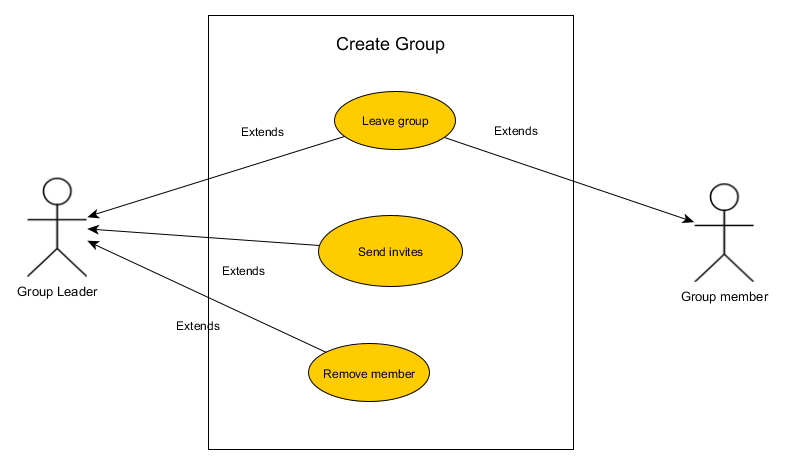
\includegraphics[scale=.5]{UseCaseCreateGroup.png}\\

\subsection{Create Group Use Case Details}

When a group is created a name has to be chosen. Once the group is created other users can be invited and therefore also remove from the group but only by the group leader.

\subsubsection{Characteristic Information}

\begin{tabular}{|l|l|}
\hline
Goal &  Create a group with the group leaders items and categories\\ \hline
Involved User & Leader of the group \\ \hline
\end{tabular}

\subsubsection{GUI to call the use case}

\begin{tabular}{|l|l|}
\hline
Input field & Valid inputs \\ \hline
 &  \\ \hline
\end{tabular}

\subsubsection{Scenario for the standard use}

\begin{tabular}{|l|l|l|}
\hline
Step & User & Activity \\ \hline
 & & \\ \hline
\end{tabular}

\subsubsection{GUIs for the standard use}

\begin{tabular}{|l|l|}
\hline
Input field & Valid inputs \\ \hline
 &  \\ \hline
\end{tabular}

\subsubsection{Scenarios for non-standard uses}

\begin{tabular}{|l|l|l|}
\hline
Step & User & Activity \\ \hline
 & & \\ \hline
\end{tabular}

\subsubsection{GUIs for the non-standard uses}

\begin{tabular}{|l|l|}
\hline
Input field & Valid inputs \\ \hline
 &  \\ \hline
\end{tabular}

\subsubsection{Workflow}

\subsection{Use Case Create Shopping list}

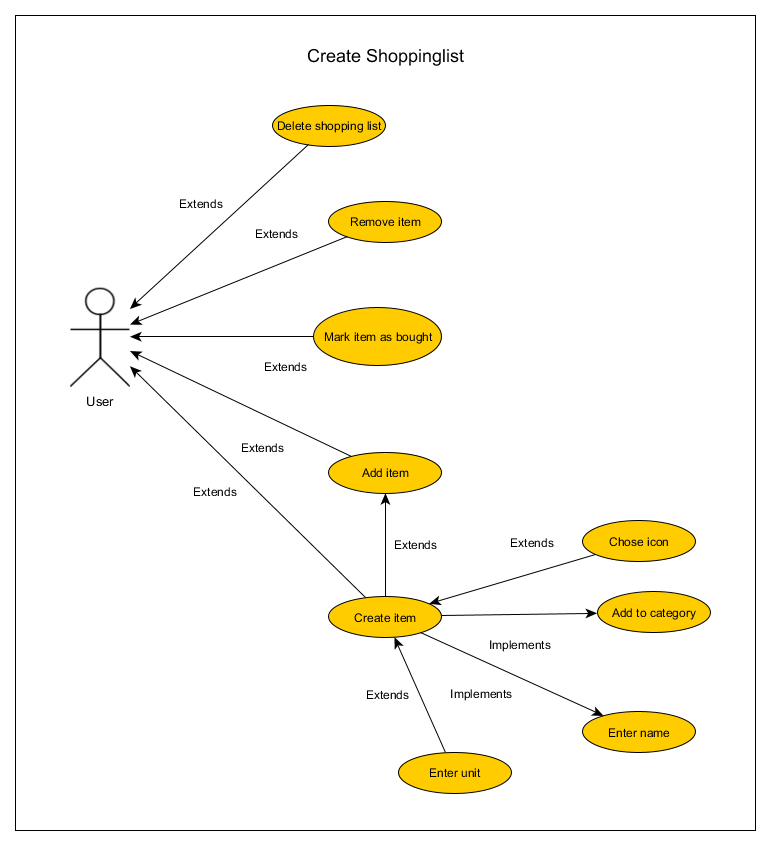
\includegraphics[scale=.5]{UseCaseCreateShoppinglist.png}\\

\subsection{Create Shopping list Use Case Details}

When creating a shopping list there are no necessary action. After the creation of the shopping list items can be added from the users personal items. When the required item is not found in the users item list it can created on the fly. In the shopping list the items are sorted by category which can be altered by the user. The items on the shopping list can be marked as bought those will be moved to the bottom of list so they do not get in the way. All bought items can be removed from the shopping list all at once. Items can also be removed. Items can also be created without a shopping list. When an item is created a name and its category has to be chosen. The user is able to choose an icon and a unit for the item.

\subsubsection{Characteristic Information}

\begin{tabular}{|l|l|}
\hline
Goal & Create an empty shopping list \\ \hline
Involved User &  User who wants to create a shopping list \\ \hline
\end{tabular}


\subsubsection{GUI to call the use case}

\begin{tabular}{|l|l|}
\hline
Input field & Valid inputs \\ \hline
 &  \\ \hline
\end{tabular}

\subsubsection{Scenario for the standard use}

\begin{tabular}{|l|l|l|}
\hline
Step & User & Activity \\ \hline
 & & \\ \hline
\end{tabular}

\subsubsection{GUIs for the standard use}

\begin{tabular}{|l|l|}
\hline
Input field & Valid inputs \\ \hline
 &  \\ \hline
\end{tabular}

\subsubsection{Scenarios for non-standard uses}

\begin{tabular}{|l|l|l|}
\hline
Step & User & Activity \\ \hline
 & & \\ \hline
\end{tabular}

\subsubsection{GUIs for the non-standard uses}

\begin{tabular}{|l|l|}
\hline
Input field & Valid inputs \\ \hline
 &  \\ \hline
\end{tabular}

\subsubsection{Workflow}

\pagebreak

\section{Non-functional Requirements}

\pagebreak

\section{Quantity Structure}

Every user has a nickname, password and e-mail. All configuration from every user concerning items, shopping lists and recipes will be saved in order to be independent of devices. Every recipe that is created inside of a group will be added to ones recipe book. A group has its own items, shopping lists and recipes it also has every member. A new user with the default configuration will use about 60 records. Considering the amount of data we chose to save the user data in a database. 

\pagebreak

\section{System Architecture and Interfaces}

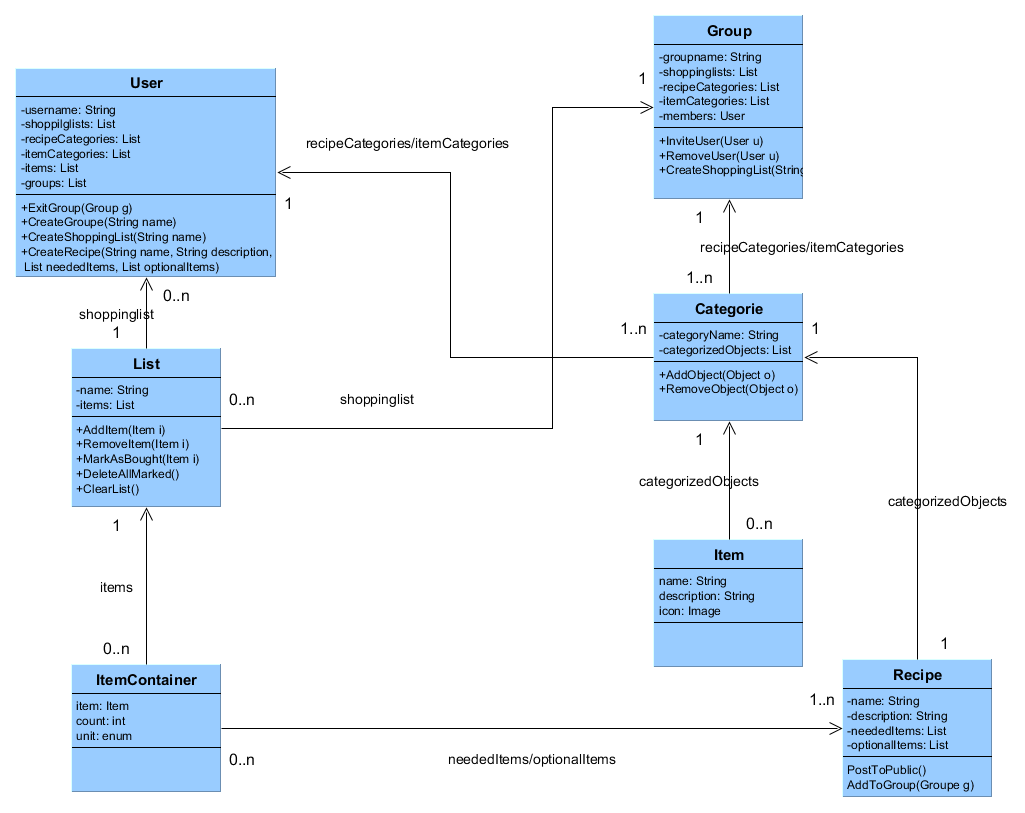
\includegraphics[scale=.5]{UMLClassDiagram.png}

\pagebreak

\section{Acceptance Criteria}

\subsection{AC001}

\begin{tabular}{|l|l|}
\hline 
\cellcolor[gray]{0.5}\textcolor{white}{Test step} & \cellcolor[gray]{0.5}\textcolor{white}{Expected behaviour} \\ \hline
Store a recipe without entering a name & Recipe will not be stored \\ 
 & and the user will be asked for a name \\ \hline
Add a picture to the recipe & Picture is visible \\
 & in the recipe book \\ \hline
Add picture to recipe & Picture is visible to all group members\\
which is stored in a group & and recipe is in the private \\ 
& recipe book \\ \hline
Storing a recipe that & Recipe will be found in the recipe book\\
has been posted & and all needed items will be created\\ \hline
\end{tabular}


\subsection{AC002}

\begin{tabular}{|l|l|}
\hline
\cellcolor[gray]{0.5}\textcolor{white}{Test step} & \cellcolor[gray]{0.5}\textcolor{white}{Expected behaviour} \\ \hline
Create a group without entering a name & Group will not be created \\ 
 & and the user will be asked for a name \\ \hline
Send invite to other user & Other user receives the invite \\
& and can join the group \\ \hline
Send invite to non-existing user & No invite will be sent and the user is told \\
& that the user does not exist \\ \hline
User other than the group leader invites a user & User should be \\ & prevented from sending the invite \\ \hline
Remove user of a group & User can no longer access group information \\
& and the removed user will be notified \\ \hline
Remove user the does not exist & Group leader will be prevented\\ \hline
User other than the group leader removes a user & The user will be prevented \\ \hline
Group leader leaves the group & The group leader must assign \\
& the next group leader \\ \hline
User leaves group & User has no longer access to group information \\ \hline
\end{tabular}

\subsection{AC003}

\begin{tabular}{|l|l|}
\hline
\cellcolor[gray]{0.5}\textcolor{white}{Test step} & \cellcolor[gray]{0.5}\textcolor{white}{Expected behaviour} \\ \hline
Creating an shopping list without entering a name & shopping list will not be created \\ 
 & and the user will be asked for a name \\ \hline
Remove item from shopping list & Item is not in list any more \\ \hline
Mark item as bought & Item will be marked \\
& and moved to the bottom of the list \\ \hline
Add existing item to shopping list & Item will be added to \\
& the list in the right category \\ \hline
Add non-existing item to shopping list & User will be asked if they \\
& want to create the item \\ \hline
Delete shopping list & Shopping list will be deleted \\ \hline
Remove bought items & Every item in the shopping list \\
& that is marked as bought will be removed \\ \hline
Creating an item without entering a name & Item will not be created \\ 
 & and the user will be asked for a name \\ \hline

\end{tabular}

\pagebreak

\end{document}  